\documentclass[a4paper]{article}
\usepackage{fontspec}
\usepackage{fontenc}
\usepackage{extarrows}
\usepackage{chemfig}
\usepackage[version=4]{mhchem}
\usepackage{mwe}
\usepackage{amsmath}
\usepackage{fancyhdr}
\usepackage{graphicx}
\usepackage{color}
\usepackage{varwidth}
\usepackage{amssymb}
\usepackage{siunitx}
\usepackage{bigfoot}
\usepackage{fancyvrb}
\usepackage{expl3}
\usepackage{calc}
\usepackage{geometry}
\geometry{left=2.5cm,right=2.5cm,top=2cm,bottom=3cm}
\setmainfont{Hiragino Sans GB}

\title{物质结构与性质}
\author{胡译文}
\date{\today}

\makeatletter
\newcommand{\figcaption}{\def@captype{figure}\caption}
\newcommand{\tabcaption}{\def@captype{table}\caption}
\makeatother

\XeTeXlinebreaklocale "zh"
\XeTeXlinebreakskip = 0pt plus 1pt

\usepackage{hyperref}
\renewcommand\contentsname{目录}

\begin{document}
	\maketitle
	\begin{center}
		若有bug请到{\color{red}\href{https://github.com/huyiwen/Chem}{github}}上提Issue。\\
		技术有限所有方程式的等号都用箭头代替了。
	\end{center}
	\renewcommand\contentsname{目录}
	\tableofcontents
	
	
	\clearpage
	\section*{Flashback}
	\subsection{元素周期表}
	\begin{itemize}
		\item 横行(周期)
		\begin{itemize}
			\item 短周期
			\begin{itemize}
				\item 一:2
				\item 二:8
				\item 三:8
			\end{itemize}
			\item 长周期
			\begin{itemize}
				\item 四:18
				\item 五:18
				\item 六:32
				\item 七:32
				\item (八:50)
			\end{itemize}
		\end{itemize}
		\item 纵列(族)
		\begin{itemize}
			\item 主族:$IA$~$VIIA$
			\item 副族:$IB$~$VIIB$
			\item $VIII$族:三列
			\item 〇族:稀有气体
		\end{itemize}
	\end{itemize}
	\subsection{元素周期律}
	\subsubsection{$IA$族(碱金属)}
	\begin{minipage}{0.48\linewidth}
		\begin{enumerate}
			\item \ce{Li}:\fbox{+3}$\;2\;1$
			\item \ce{Na}:\fbox{+11}$\;2\;8\;1$
			\item \ce{K}:\fbox{+19}$\;2\;8\;8\;1$
			\item \ce{Rb}:\fbox{+37}$\;2\;8\;18\;8\;1$
			\item \ce{Cs}:\fbox{+55}$\;2\;8\;18\;18\;8\;1$
		\end{enumerate}
	\end{minipage}
	\hfill
	\begin{minipage}{.48\linewidth}
		从上至下:
		\begin{itemize}
			\item 电子层数$\;\uparrow$
			\item 原子半径$\;\uparrow$
			\item 原子核对最外层电子吸引力$\;\downarrow$
			\item 失电子能力$\;\uparrow$
			\item 金属性$\;\uparrow$
			\item 与酸(水)反应剧烈程度$\;\uparrow$
			\item 最高价氧化物对应水化物的碱性$\;\uparrow$
		\end{itemize}
	\end{minipage}
	\begin{itemize}
		\item 金属性:$\ce{Li}<\ce{Na}<\ce{K}<\ce{Rb}<\ce{Cs}$
		\item 氧化性:$\ce{Li+}<\ce{Na+}<\ce{K+}<\ce{Rb+}<\ce{Cs+}$
		\item 碱性:$\ce{LiOH}<\ce{NaOH}<\ce{KOH}<\ce{RbOH}<\ce{CsOH}$
	\end{itemize}
	
	\subsubsection{$IIA$族(碱土元素)}
	\begin{minipage}{0.48\linewidth}
		\begin{enumerate}
			\item \ce{Be}:\fbox{+4}$\;2\;2$
			\item \ce{Mg}:\fbox{+12}$\;2\;8\;2$
			\item \ce{Ca}:\fbox{+20}$\;2\;8\;8\;2$
			\item \ce{Sr}:\fbox{+38}$\;2\;8\;18\;8\;2$
			\item \ce{Ba}:\fbox{+56}$\;2\;8\;18\;18\;8\;2$
		\end{enumerate}
	\end{minipage}
	\hfill
	\begin{minipage}{.48\linewidth}
		从上至下:
		\begin{itemize}
			\item 电子层数$\;\uparrow$
			\item 原子半径$\;\uparrow$
			\item 原子核对最外层电子吸引力$\;\downarrow$
			\item 失电子能力$\;\uparrow$
			\item 金属性$\;\uparrow$
			\item 与酸(水)反应剧烈程度$\;\uparrow$
			\item 最高价氧化物对应水化物的碱性$\;\uparrow$
		\end{itemize}
	\end{minipage}
	\begin{itemize}
		\item 金属性:$\ce{Cs}>\ce{Ba}>\ce{Rb}>\ce{Sr}>\ce{K}>\ce{Ca}>\ce{Na}>\ce{Mg}>\ce{Li}>\ce{Be}$
	\end{itemize}
	
	\subsubsection{$VIIA$族(卤素)}
	\begin{minipage}{0.48\linewidth}
		\begin{enumerate}
			\item \ce{F}:\fbox{+9}$\;2\;7$
			\item \ce{Cl}:\fbox{+17}$\;2\;8\;7$
			\item \ce{Br}:\fbox{+35}$\;2\;8\;8\;7$
			\item \ce{I}:\fbox{+53}$\;2\;8\;18\;8\;7$
		\end{enumerate}
	\end{minipage}
	\hfill
	\begin{minipage}{.48\linewidth}
		从上至下:
		\begin{itemize}
			\item 电子层数$\;\uparrow$
			\item 原子半径$\;\uparrow$
			\item 原子核对最外层电子吸引力$\;\downarrow$
			\item 得电子能力$\;\downarrow$
			\item 非金属性$\;\downarrow$
			\item 与\ce{H2}反应剧烈程度$\;\downarrow$
			\item 最高价氧化物对应水化物的酸性$\;\downarrow$
		\end{itemize}
	\end{minipage}
	\begin{itemize}
		\item 非金属性:$\ce{F}>\ce{Cl}>\ce{Br}>\ce{I}$
		\item 氧化性:$\ce{F2}>\ce{Cl2}>\ce{Br2}>\ce{I2}$
		\item 酸性:$\ce{HClO4}>\ce{HBrO4}>\ce{HIO4}$
		\item 酸性:$\ce{HF}<\ce{HCl}<\ce{HBr}<\ce{HI}$(气态氢化物稳定性)
	\end{itemize}
	
	\subsubsection{第三周期}
	\begin{minipage}{1\linewidth}
	\ce{Na}\;\ce{Mg}\;\ce{Al}\quad\ce{Si}\;\ce{P}\;\ce{S}\;\ce{Cl}
	\end{minipage}
	$\left\{\begin{array}{lr}
		\ce{SiH4 + O2 ->[{自燃}] SiO2 + H2O}\\
		\ce{PH3 + 2O2 ->[{点燃}] H3PO4}\\
		\ce{H2S + O2 ->[{点燃}] SO2 + H2O}\\
		\ce{HCl + O2 ->[{高温}] Cl2 + H2O}\\
	\end{array}\right.$
	
	
	\clearpage
	\section{原子结构}
	
	
	\subsection{发现史}
	\begin{itemize}
		\item 道尔顿:原子说
		\item JJ-汤姆逊:电子
		\item 卢瑟福:核式结构
		\item 玻尔:行星模型
		\item 量子科学家:电子云模型(电子出现的概率统计)
	\end{itemize}
	
	
	\subsection{能层和能级}
	\paragraph{能层}
	能层又叫电子层,在含有多个电子的原子内,电子分别在能量不同的区域内运动,这种不同的区域就是能层。由于原子中的电子是处在原子核的引力场中,电子总是尽可能先从内层排起,当一层充满后再填充下一层。
	\paragraph{能级}
	能级又叫电子亚层,同一个能层的电子,能量也可能不同,又可以把他们分成不同能级。
	\begin{figure}[h]
	\centering
	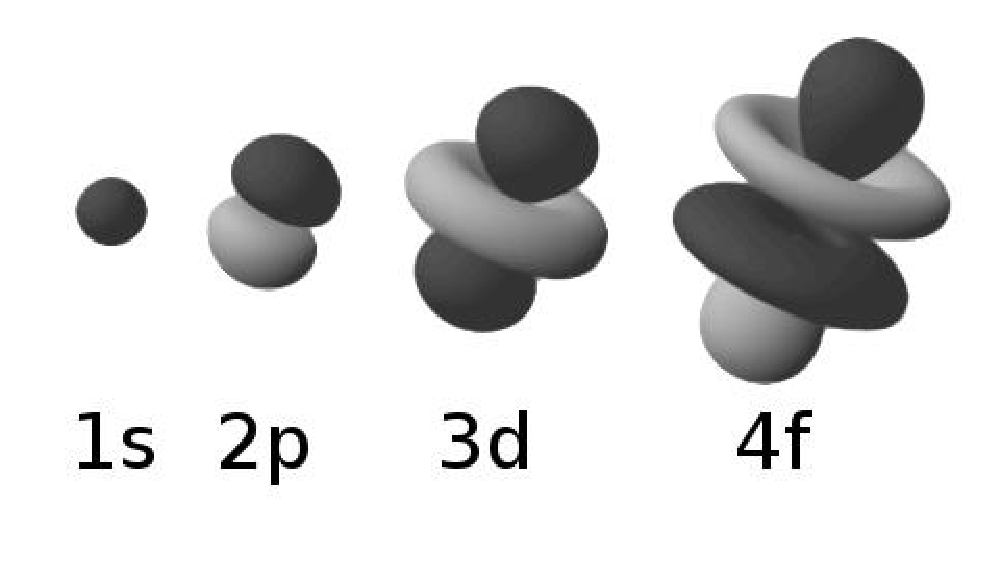
\includegraphics[scale=0.4]{res/Orbital.pdf}
	\end{figure}
	
	\subsection{四个量子数}	
	\subsubsection{主量子数}
	主量子数$n$,由周期数决定
	$$n=1,2,3,4,5...$$
	\renewcommand\arraystretch{2}
	\begin{center}
	\begin{tabular}{|c|c|c|c|c|c|}
		\hline
		$n$ & $1$ & $2$ & $3$ & $4$ & $5$\\\hline
		能层 & $K$ & $L$ & $M$ & $N$ & $O$\\\hline
	\end{tabular}
	\end{center}
	\subsubsection{角量子数}
	角量子数$l$,由能级决定
	$$l=0,1,2,3,4,5...$$
	\begin{center}
	\begin{tabular}{|c|c|c|c|c|c|c|}
		\hline
		$l$ & $0$ & $1$ & $2$ & $3$ & $4$ & $5$\\\hline
		能级 & $s$ & $p$ & $d$ & $f$ & $g$ & $h$\\\hline
	\end{tabular}
	\end{center}
	\paragraph{各个能层含有的能级}
	\begin{center}
	\begin{tabular}{|c|c|c|c|c|c|c|c|c|c|c|c|}
		\hline
		能层 & $K$ & \multicolumn{2}{c|}{$L$} & \multicolumn{3}{c|}{$M$} & \multicolumn{4}{c|}{$N$}\\\hline
		$n$ & $1$ & \multicolumn{2}{c|}{$2$} & \multicolumn{3}{c|}{$3$} & \multicolumn{4}{c|}{$4$}\\\hline
		$l$ & $0$ & $0$ & $1$ & $0$ & $1$ & $2$ & $0$ & $1$ & $2$ & $3$\\\hline
		能级 & $1s$ & $2s$ & $2p$ & $3s$ & $3p$ & $3d$ & $4s$ & $4p$ & $4d$ & $4f$\\\hline
	\end{tabular}
	\end{center}
	\subsubsection{磁量子数}
	磁量子数$m$,决定轨道数
	$$m=0,\pm1,\pm2,...,\pm l$$
	\begin{center}
	\begin{tabular}{|c|c|c|c|c|c|c|c|}
		\hline
		能层 & $K$ & \multicolumn{2}{c|}{$L$} & \multicolumn{3}{c|}{$M$}\\\hline
		$n$ & $1$ & \multicolumn{2}{c|}{$2$} & \multicolumn{3}{c|}{$3$}\\\hline
		$l$ & $0$ & $0$ & $1$ & $0$ & $1$ & $2$\\\hline
		$m$ & $0$ & $0$ & $0/+1/-1$ & $0$ & $0/+1/-1$ & $0/+1/-1/+2/-2$\\\hline
		轨道数 & 1 & 1 & 3 & 1 & 3 & 5\\\hline
		电子排布式 & $1s$ & $2s$ & $2p$ & $3s$ & $3p$ & $3d$\\\hline
		轨道表达式 & \fbox{$\ \ $} & \fbox{$\ \ $} & \fbox{$\ \ $}\fbox{$\ \ $}\fbox{$\ \ $} & \fbox{$\ \ $} & \fbox{$\ \ $}\fbox{$\ \ $}\fbox{$\ \ $} & \fbox{$\ \ $}\fbox{$\ \ $}\fbox{$\ \ $}\fbox{$\ \ $}\fbox{$\ \ $}\\\hline
	\end{tabular}
	\end{center}
	\subsubsection{自旋量子数}
	自旋量子数$m_s$,决定电子运动方向(共两种情况,在轨道表达式中分别为上、下箭头)
	$$m_s=\pm\frac12$$
	
	
	\subsection{电子、价电子排布式和轨道表达式}
	\paragraph{相关概念}
	\subparagraph{价电子}
	价电子指原子核外电子中能与其他原子相互作用形成化学键的电子,为原子核外跟元素化合价有关的电子
	\subparagraph{轨道表达式}
	又叫电子排布图
	\paragraph{$\ce{_{26}Fe}$}
	\begin{itemize}
		\item 电子排布式:$1s^2\,2s^2\,2p^6\,3s^2\,3p^6\,3d^6\,4s^2$
		\item 价电子排布式:$3d^6\,4s^2$
		\item 电子轨道表达式:\fbox{$\uparrow\downarrow$}\quad\fbox{$\uparrow\downarrow$}\quad\fbox{$\uparrow\downarrow$}\fbox{$\uparrow\downarrow$}\fbox{$\uparrow\downarrow$}\quad\fbox{$\uparrow\downarrow$}\quad\fbox{$\uparrow\downarrow$}\fbox{$\uparrow\downarrow$}\fbox{$\uparrow\downarrow$}\quad\fbox{$\uparrow\downarrow$}\fbox{$\uparrow\ $}\fbox{$\uparrow\ $}\fbox{$\uparrow\ $}\fbox{$\uparrow\ $}\quad\fbox{$\uparrow\downarrow$}
		\item 价电子轨道表达式:\fbox{$\uparrow\downarrow$}\fbox{$\uparrow\ $}\fbox{$\uparrow\ $}\fbox{$\uparrow\ $}\fbox{$\uparrow\ $}\quad\fbox{$\uparrow\downarrow$}
	\end{itemize}
	
	

	\subsection{徐光宪规则}
	根据实验总结出的计算能级高低的近似规则
	$$E=n+0.7l$$
	\begin{itemize}
		\item $E(4s)=4+0.7\times 0=4$
		\item $E(3d)=3+0.7\times 2=4.4$
	\end{itemize}


	\subsection{电子排布原理}
	\subsubsection{能量最低原理}
	电子尽量填充至能量低的轨道中
	\begin{itemize}
		\item 注意:同一能级中的轨道(如$3p$中的 \fbox{$\ \ $}\fbox{$\ \ $}\fbox{$\ \ $} )能量相等
	\end{itemize}
	\subsubsection{泡利不相容原理}
	一个轨道中不能存在自旋相同的电子(轨道表达式中同轨道箭头方向不同)
	\begin{itemize}
		\item \fbox{$\uparrow\ $}:正确
		\item \fbox{$\ \downarrow$}:正确
		\item \fbox{$\uparrow\downarrow$}:正确
		\item \fbox{$\uparrow\uparrow$}:错误
	\end{itemize}
	\subsubsection{洪特规则}
	电子总是先填充空轨道
	\begin{enumerate}
		\item \fbox{$\uparrow\ $}\fbox{$\ \ $}\fbox{$\ \ $}\footnote{这些方格应该是一样大的,但是技术有限就只能这样}
		\item \fbox{$\uparrow\ $}\fbox{$\uparrow\ $}\fbox{$\ \ $}
		\item \fbox{$\uparrow\ $}\fbox{$\uparrow\ $}\fbox{$\uparrow\ $}
		\item \fbox{$\uparrow\downarrow$}\fbox{$\uparrow\ $}\fbox{$\uparrow\ $}
		\item \fbox{$\uparrow\downarrow$}\fbox{$\uparrow\downarrow$}\fbox{$\uparrow\ $}
		\item \fbox{$\uparrow\downarrow$}\fbox{$\uparrow\downarrow$}\fbox{$\uparrow\downarrow$}
	\end{enumerate}
	\paragraph{洪特特例}
	各轨道电子排布为全满、半满或全空时有特殊的稳定性。(主要出现在过渡元素)
	\subparagraph{\ce{_24Cr}}
	\begin{itemize}
		\item 稳定:$1s^2\,2s^2\,2p^6\,3s^2\,3p^6\,\underbrace{3d^5\,4s^1}_{半满}$
		\item 不稳定:$1s^2\,2s^2\,2p^6\,3s^2\,3p^6\,3d^4\,4s^2$
	\end{itemize}
	\vskip 10mm
	\subparagraph{\ce{_26Fe}}
	\begin{itemize}
		\item \ce{Fe}:$1s^2\,2s^2\,2p^6\,3s^2\,3p^6\,3d^6\,4s^2$
		\item \ce{Fe2+}:$1s^2\,2s^2\,2p^6\,3s^2\,3p^6\,3d^6$
		\item \ce{Fe3+}:$1s^2\,2s^2\,2p^6\,3s^2\,3p^6\,\underbrace{3d^5}_{更稳定}$
	\end{itemize}
	\subsubsection{构造原理}
	根据构造原理,绝大多数基态原子核外电子的排布都遵循下列顺序(徐光宪规则计算):\\
	$1s$、$2s$、$2p$、$3s$、$3p$、$4s$、$3d$、$4p$、$5s$、$4d$、$5p$、$6s$、$4f$、$5d$......
	\begin{figure}[h]
	\centering
	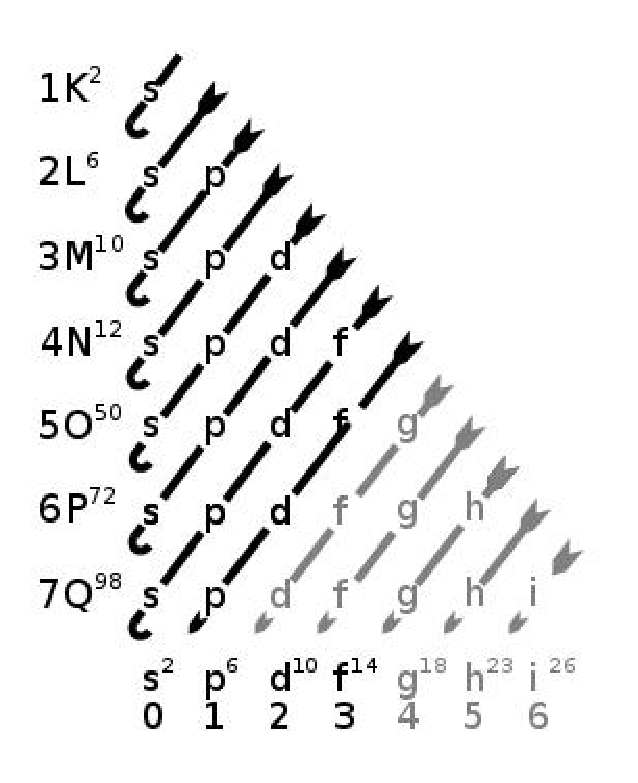
\includegraphics[scale=0.6]{res/Aufbau.pdf}
	\end{figure}
	
	\subsection{电子跃迁}
	\subsubsection{原子光谱}
	原子光谱,是由原子中的电子在能量变化时所发射或吸收的一系列波长的光所组成的光谱。
	\begin{itemize}
		\item \ce{Na}:$1s^2\,2s^2\,2p^6\,3s^1$ 基态
		\item \ce{Na}:$1s^2\,2s^2\,2p^5\,3s^2$ 激发态
	\end{itemize}
	\paragraph{原子发射光谱}
	在热激发或电激发下,从激发态回到基态时发射的特征谱。
	\paragraph{原子吸收光谱}
	当光的入射辐射的频率等于电子由基态跃迁到较高能态(一般是第一激发态)所需能量频率时,原子中的外层电子将选择性地吸收其同种元素所发射的特征谱线。如焰色反应。
	
	
	\clearpage
	\section{元素的性质}
	
	
	\subsection{元素周期表分区}
	按照价电子所在能级分区。
	\begin{figure}[h]
	\centering
	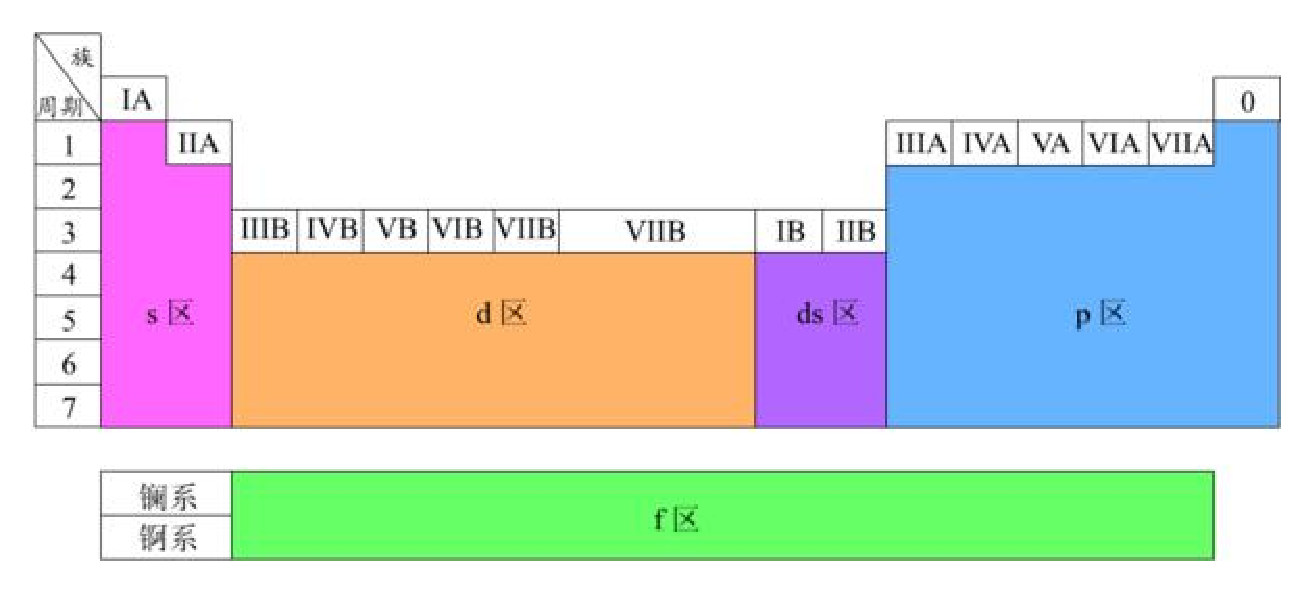
\includegraphics[scale=0.5]{res/Ptable.pdf}
	\end{figure}
	
	
	\subsection{电负性}
	\subsubsection{定义}
	用来衡量元素得失电子能力的物理量。
	\begin{figure}[h]
	\centering
	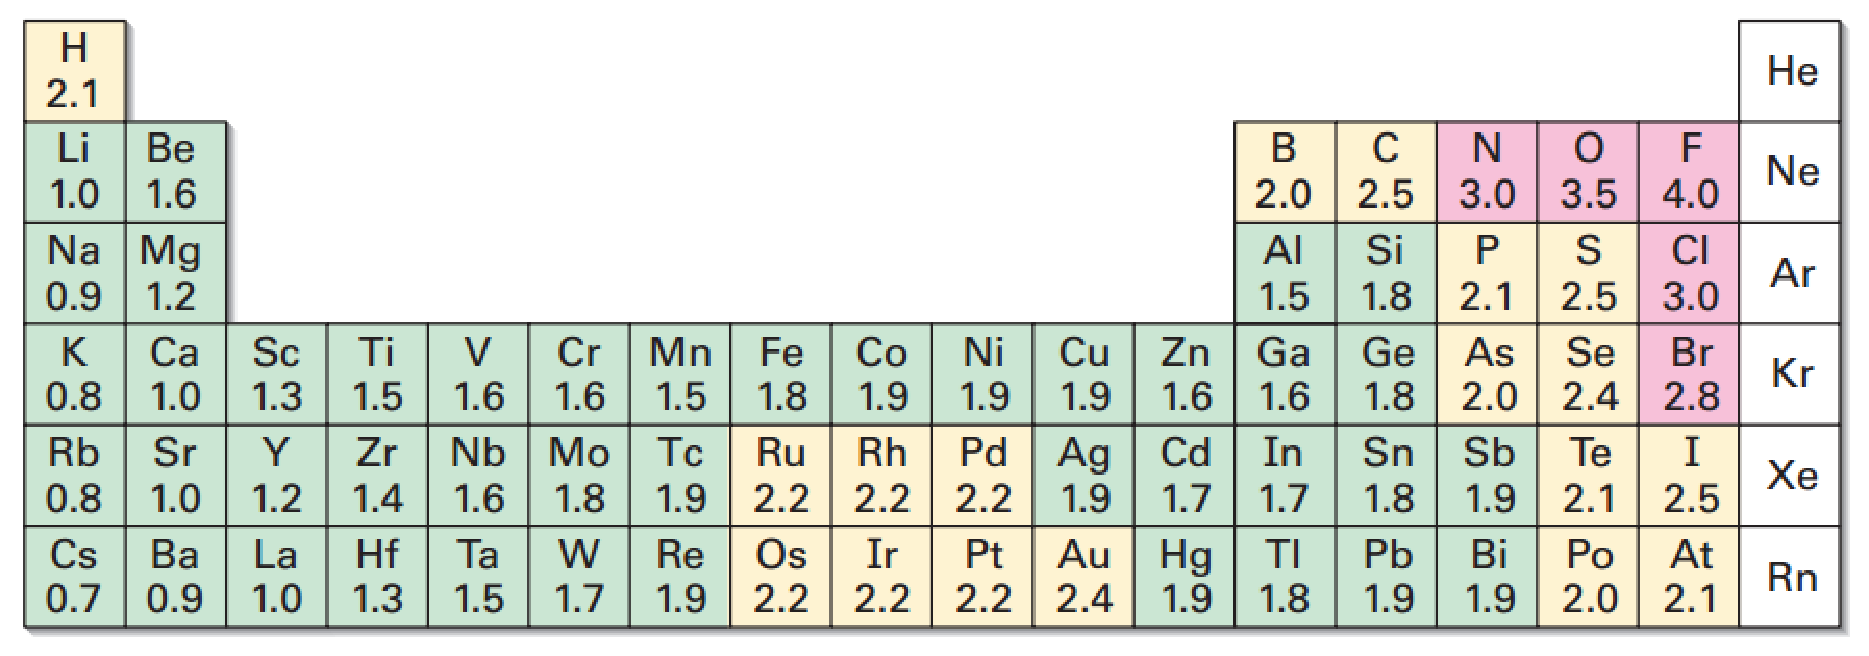
\includegraphics[scale=0.5]{res/EN.pdf}
	\end{figure}
	\begin{itemize}
		\item \ce{F}的电负性最大:4.0
		\item \ce{Cs}的电负性最小:0.7
	\end{itemize}
	
	\subsubsection{应用}
	\paragraph{判断水解产物}
	
	\hfill
	\begin{figure}[h]
	\begin{minipage}{0.48\linewidth}
	\begin{itemize}
		\item $\ce{SiCl4 + 3H2O ->[\Delta] H2SiO3 + 4HCl}$
		\item $\ce{NCl3 + 3H2O -> NH3 + 3HClO}$
	\end{itemize}
	\end{minipage}
	\begin{minipage}{0.48\linewidth}
	\centering
	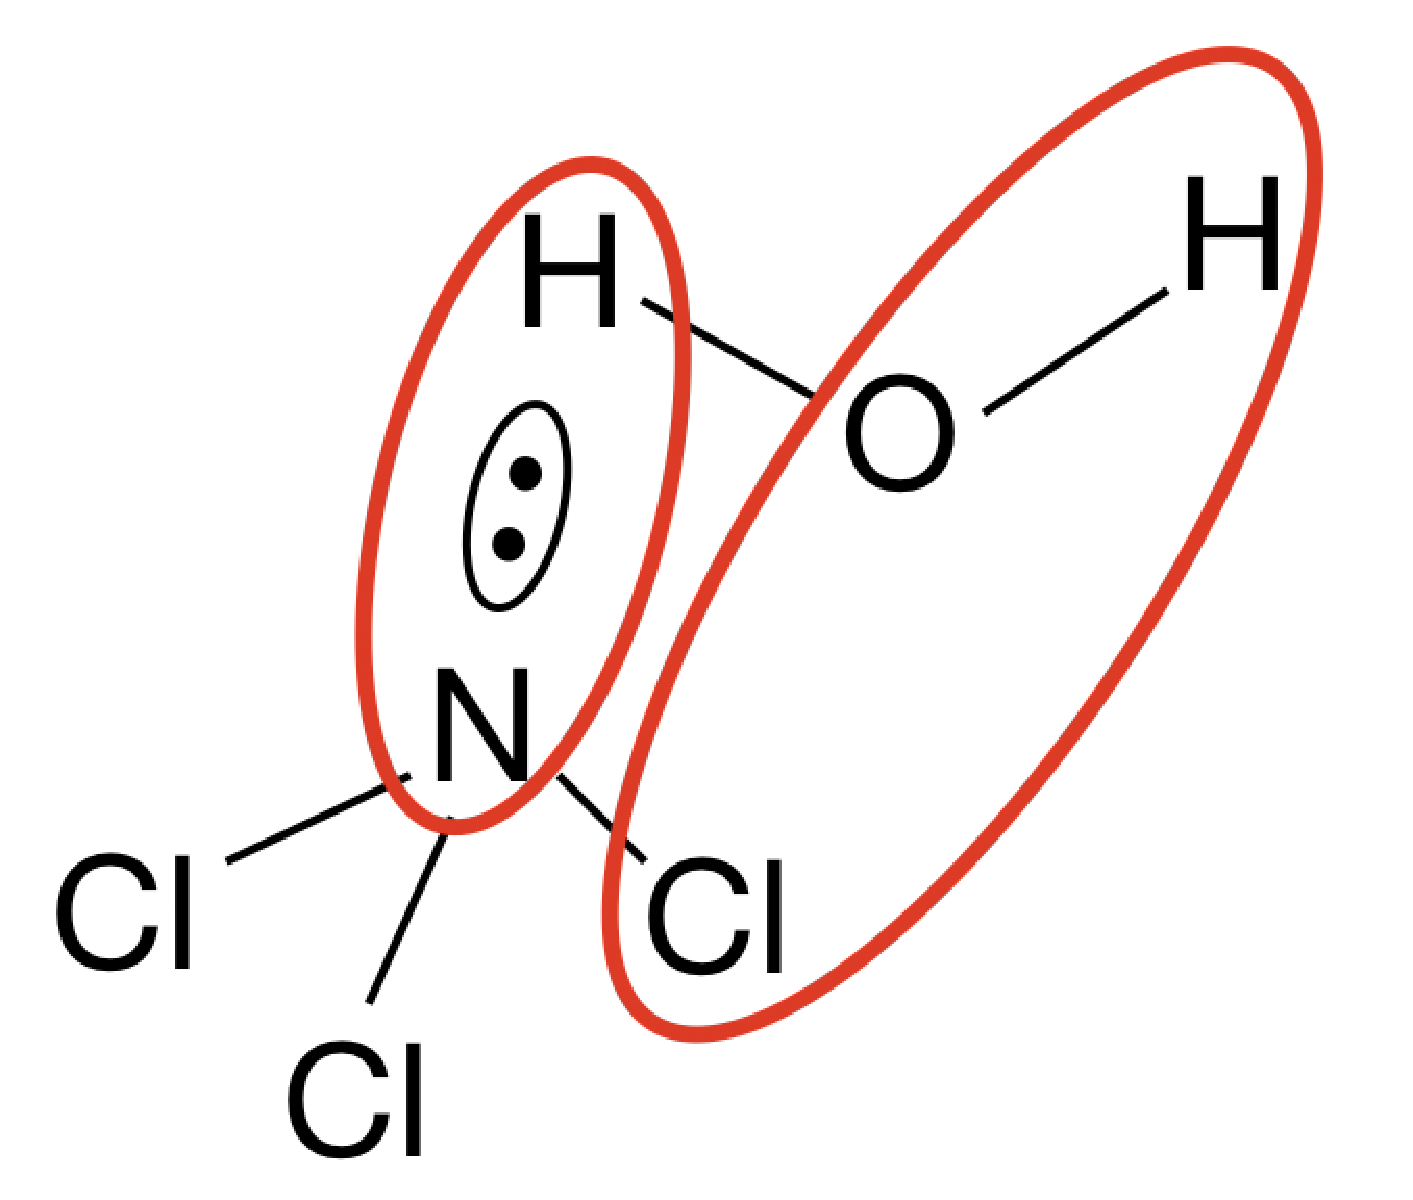
\includegraphics[scale=0.2]{res/NCl.pdf}
	\end{minipage}
	\end{figure}
	\paragraph{判断元素化合价}
	$$\mathop{H}^{+1}\mathop{Cl}^{+1}\mathop{O}^{-2}:\ce{H-O-Cl}$$
	$$\mathop{H}^{+1}\mathop{F}^{-1}\mathop{O}^{0}:\ce{H-O-F}$$
	\paragraph{判断化学键类型}
	一般而言电负性之差大于 $1.7$ 的元素之间形成离子键,小于 $1.7$ 的形成共价键
	
	
	\subsection{电子亲和能}
	\subsubsection{定义}
	气态原子得到一个电子、生成相应离子吸收/放出的能量。
	$$\ce{M(g) + e- -> M- (g)\qquad \Delta H}$$
	\begin{tabular}{|c|c|}
	\hline
	电子亲和能 & 能量变化\\\hline
	$>0$ & 放热\\\hline
	$<0$ & 吸热\\\hline
	\end{tabular}
	\begin{itemize}
		\item 电子亲和能最大的是\ce{Cl}(\ce{F}半径过小导致得电子后过于拥挤,电子间排斥力大,氟离子稳定性相对较差)
	\end{itemize}
	
	
	\subsection{电离能}
	\subsubsection{定义}
	气态原或离子失去电子形成气态离子所吸收的能量。
	\paragraph{代号}
	$I_n$:第 $n$ 电离能(失去 $n$ 个电子)。第一电离能可以省略 $1$ 。
	\paragraph{单位}
	$KJ/mol$
	\subsubsection{应用}
	\begin{itemize}
		\item 同周期中,$IA$族元素是 $I_1$ 最小的、$O$族元素最大
		\item 除放射性元素中:
		$$\max(I_1)=\ce{He}\qquad\max(I_2)=\ce{Li}$$
		$$\min(I_1)=\ce{Cs}\qquad\min(I_2)=\ce{Ba}$$
		\item 测定最外层电子数:\ce{Mg}:$I_1<I_2<<I_3$
		\item 第二周期 $I_1$ 变化规律:
		$$\mathop{\ce{Li}}_{2s^1}\quad\mathop{\ce{Be}}_{2s^2}\quad\mathop{\ce{B}}_{2s^2\,2p^1}\quad\mathop{\ce{C}}_{2s^2\,2p^2}\quad\mathop{\ce{N}}_{2s^2\,2p^3}\quad\mathop{\ce{O}}_{2s^2\,2p^4}\quad\mathop{\ce{F}}_{2s^2\,2p^5}$$
		\begin{figure}[h]
		\centering
		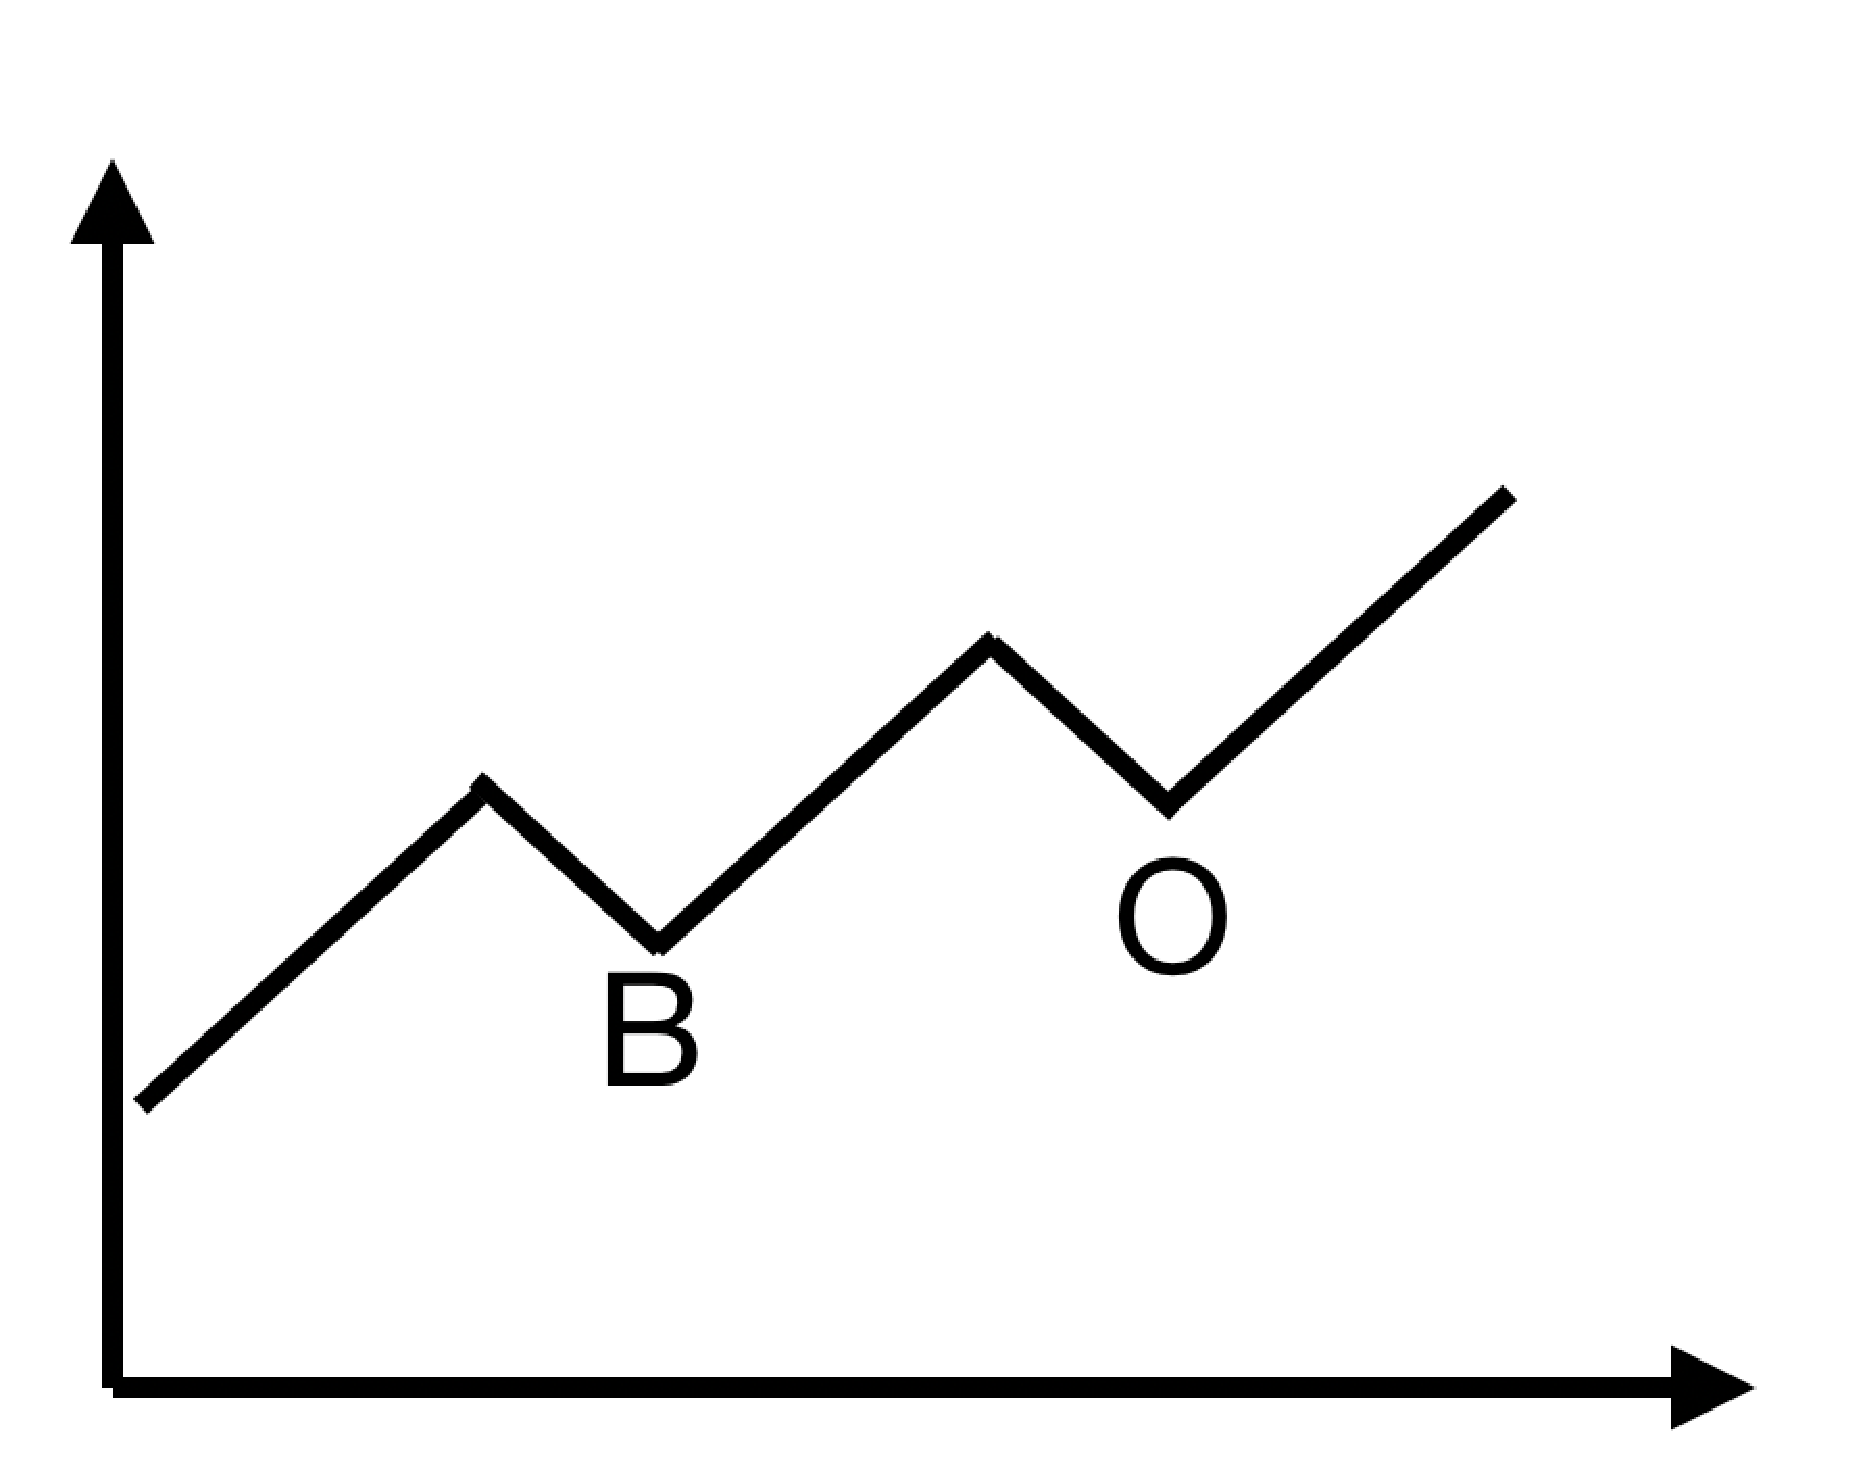
\includegraphics[scale=0.12]{res/I1.pdf}
		\end{figure}
	\end{itemize}
	
	
	\subsection{对角线规则}
	$$
	\ce{Li}-\ce{Mg}\qquad\ce{Be}-\ce{Al}\qquad\ce{B}-\ce{Si}
	$$
	\begin{itemize}
		\item $\left\{\begin{array}{lr}
				\ce{Be + 2OH- -> BeO2- + H2 ^}\\
				\ce{2Al + 2OH- + 2H2O -> 2AlO2- + 3H2 ^}\\
			\end{array}\right.$
		\item $\left\{\begin{array}{lr}
				\ce{2B + 2OH- + 2H2O -> 2BO2- + 3H2 ^}\\
				\ce{Si + 2OH- + H2O -> SiO3^2- + 2H2 ^}\\
			\end{array}\right.$
	\end{itemize}
	
	
	\clearpage
	\section{化学键}
	
	
	\subsection{分类}
	
	
	\subsection{共价键的形成}
	
	
	\subsection{键参数}
	
	
	\subsection{配合物}
	
	
	\clearpage
	\section{分子结构}
	
	
	\subsection{Lewis结构式}
	
	
	\subsection{中心原子轨道杂化理论}
	
	
	\subsection{VSPER构型}
	
	
	\subsection{立体构型}
	
	
	\clearpage
	\section{分子的性质}
	
	
	\subsection{分子极性}
	
		
	\subsection{分子手性}
	
	
	\subsection{氢键}
		
	
	\clearpage
	\section{晶体结构}
	
	
	\subsection{晶体}
	
	\subsubsection{定义}
	
	\subsubsection{鉴别}
	
	\subsubsection{获取}
	
	
	\subsection{原子晶体}
	
	\subsection{分子晶体}
	
	\subsection{离子晶体}
	
	\subsubsection{晶格能}
	
	\subsubsection{金属晶体}
	
	
	\clearpage
	\section{晶体的性质以及计算}
	
	
	\subsection{熔沸点比较}
	
	\subsubsection{不同类型晶体}
	
	
	\subsubsection{相同类型晶体}
	
	
	\subsection{晶体计算}
	
	\subsubsection{晶胞的组成}
	
	\subsubsection{晶体微粒个数}
	
\end{document}